


\tikzset{every picture/.style={line width=0.75pt}} %set default line width to 0.75pt        

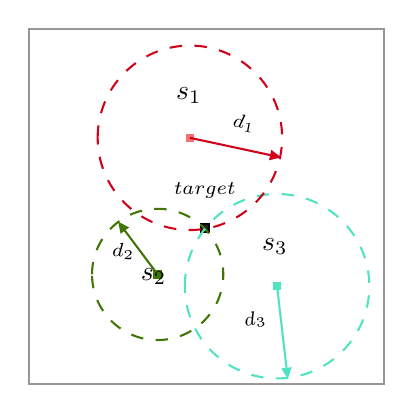
\begin{tikzpicture}[x=0.75pt,y=0.75pt,yscale=-1,xscale=1]
%uncomment if require: \path (0,300); %set diagram left start at 0, and has height of 300

%Shape: Square [id:dp3139397432452311] 
\draw  [color={rgb, 255:red, 154; green, 150; blue, 150 }  ,draw opacity=1 ] (75,51) -- (246,51) -- (246,222) -- (75,222) -- cycle ;
%Shape: Square [id:dp6615824497311407] 
\draw  [fill={rgb, 255:red, 33; green, 33; blue, 33 }  ,fill opacity=1 ] (157.96,145) -- (162,145) -- (162,149.04) -- (157.96,149.04) -- cycle ;
%Shape: Square [id:dp7238674463227524] 
\draw  [draw opacity=0][fill={rgb, 255:red, 80; green, 227; blue, 194 }  ,fill opacity=1 ] (192.64,173.04) -- (196.68,173.04) -- (196.68,177.08) -- (192.64,177.08) -- cycle ;
%Shape: Square [id:dp08550191202342461] 
\draw  [draw opacity=0][fill={rgb, 255:red, 248; green, 112; blue, 112 }  ,fill opacity=1 ] (150.64,101.54) -- (154.68,101.54) -- (154.68,105.58) -- (150.64,105.58) -- cycle ;
%Shape: Square [id:dp7141151551550344] 
\draw  [draw opacity=0][fill={rgb, 255:red, 65; green, 117; blue, 5 }  ,fill opacity=1 ] (135.1,167.36) -- (139.14,167.36) -- (139.14,171.4) -- (135.1,171.4) -- cycle ;
%Shape: Circle [id:dp9475883625678077] 
\draw  [color={rgb, 255:red, 65; green, 117; blue, 5 }  ,draw opacity=1 ][dash pattern={on 4.5pt off 4.5pt}] (105.5,169.38) .. controls (105.5,151.92) and (119.66,137.76) .. (137.12,137.76) .. controls (154.58,137.76) and (168.74,151.92) .. (168.74,169.38) .. controls (168.74,186.84) and (154.58,201) .. (137.12,201) .. controls (119.66,201) and (105.5,186.84) .. (105.5,169.38) -- cycle ;
%Shape: Circle [id:dp7445719218104008] 
\draw  [color={rgb, 255:red, 80; green, 227; blue, 194 }  ,draw opacity=1 ][dash pattern={on 4.5pt off 4.5pt}] (150.22,175.06) .. controls (150.22,150.52) and (170.12,130.62) .. (194.66,130.62) .. controls (219.2,130.62) and (239.1,150.52) .. (239.1,175.06) .. controls (239.1,199.6) and (219.2,219.5) .. (194.66,219.5) .. controls (170.12,219.5) and (150.22,199.6) .. (150.22,175.06) -- cycle ;
%Shape: Circle [id:dp34573460581909865] 
\draw  [color={rgb, 255:red, 208; green, 2; blue, 27 }  ,draw opacity=1 ][dash pattern={on 4.5pt off 4.5pt}] (108.22,103.56) .. controls (108.22,79.02) and (128.12,59.12) .. (152.66,59.12) .. controls (177.2,59.12) and (197.1,79.02) .. (197.1,103.56) .. controls (197.1,128.1) and (177.2,148) .. (152.66,148) .. controls (128.12,148) and (108.22,128.1) .. (108.22,103.56) -- cycle ;
%Straight Lines [id:da1278538436839034] 
\draw [color={rgb, 255:red, 208; green, 2; blue, 27 }  ,draw opacity=1 ]   (152.66,103.56) -- (193.65,112.37) ;
\draw [shift={(196.58,113)}, rotate = 192.13] [fill={rgb, 255:red, 208; green, 2; blue, 27 }  ,fill opacity=1 ][line width=0.08]  [draw opacity=0] (5.36,-2.57) -- (0,0) -- (5.36,2.57) -- cycle    ;
%Straight Lines [id:da7908947105774531] 
\draw [color={rgb, 255:red, 80; green, 227; blue, 194 }  ,draw opacity=1 ]   (194.66,175.06) -- (199.46,216.71) ;
\draw [shift={(199.81,219.69)}, rotate = 263.42] [fill={rgb, 255:red, 80; green, 227; blue, 194 }  ,fill opacity=1 ][line width=0.08]  [draw opacity=0] (5.36,-2.57) -- (0,0) -- (5.36,2.57) -- cycle    ;
%Straight Lines [id:da5760661930443354] 
\draw [color={rgb, 255:red, 65; green, 117; blue, 5 }  ,draw opacity=1 ]   (137.12,169.38) -- (119.9,146.38) ;
\draw [shift={(118.1,143.98)}, rotate = 53.17] [fill={rgb, 255:red, 65; green, 117; blue, 5 }  ,fill opacity=1 ][line width=0.08]  [draw opacity=0] (5.36,-2.57) -- (0,0) -- (5.36,2.57) -- cycle    ;


% Text Node
\draw (113.8,152.74) node [anchor=north west][inner sep=0.75pt]  [font=\scriptsize,rotate=-1.68] [align=left] {$\displaystyle d_{2}$};
% Text Node
\draw (176.58,186.84) node [anchor=north west][inner sep=0.75pt]  [font=\scriptsize,rotate=-351.95] [align=left] {$\displaystyle d_{3}$};
% Text Node
\draw (173.06,89.98) node [anchor=north west][inner sep=0.75pt]  [font=\scriptsize,rotate=-10.92] [align=left] {$\displaystyle d_{1}$};
% Text Node
\draw (143.5,123.5) node [anchor=north west][inner sep=0.75pt]  [font=\scriptsize] [align=left] {$\displaystyle target$};
% Text Node
\draw (186,150.5) node [anchor=north west][inner sep=0.75pt]   [align=left] {$\displaystyle s_{3}$};
% Text Node
\draw (127.5,165) node [anchor=north west][inner sep=0.75pt]   [align=left] {$\displaystyle s_{2}$};
% Text Node
\draw (144.5,78) node [anchor=north west][inner sep=0.75pt]   [align=left] {$\displaystyle s_{1}$};


\end{tikzpicture}